\documentclass{beamer}
%\documentclass[aspectratio=169]{beamer}
%
\mode<presentation>
{
  \usetheme{default}      
  \usecolortheme{default}
  \usefonttheme{default} 
  \setbeamertemplate{navigation symbols}{}
  \setbeamertemplate{caption}[numbered]
} 

\usepackage[english]{babel}
\usepackage[utf8x]{inputenc}
\usepackage{bbm}

\newcommand{\1}[1]{\mathbbm{1}\left[#1\right]}
\newcommand{\norm}[1]{\left\lVert#1\right\rVert}
\newcommand{\yi}{y^{(i)}}
\newcommand{\yhat}{\hat{y}}
\newcommand{\yhati}{\hat{y}^{(i)}}

\title{Machine learning from scratch}
\subtitle{Lecture 6: Non-linear models, parameter selection}
\author{Alexis Zubiolo\newline\texttt{alexis.zubiolo@gmail.com}}
\institute{Data Science Team Lead @ Adcash}
\date{March 9, 2017}

\begin{document}

\begin{frame}
  \titlepage
\end{frame}

\begin{frame}{Course outline}
Last time, we reviewed the main ideas behind OLS
\vfill
\pause
This lecture will go a bit further by introducing:
\begin{itemize}
	\item Non linear models (polynomial kernels)
	\item Model evaluation
	\item Parameter selection
\end{itemize}
\end{frame}

\begin{frame}
	\center
	\huge{More complex models}
\end{frame}

\begin{frame}{Outliers and overfitting}
Recall from previous course: Outliers can ruin the trained model.
\pause
\vfill
\begin{figure}
\centering
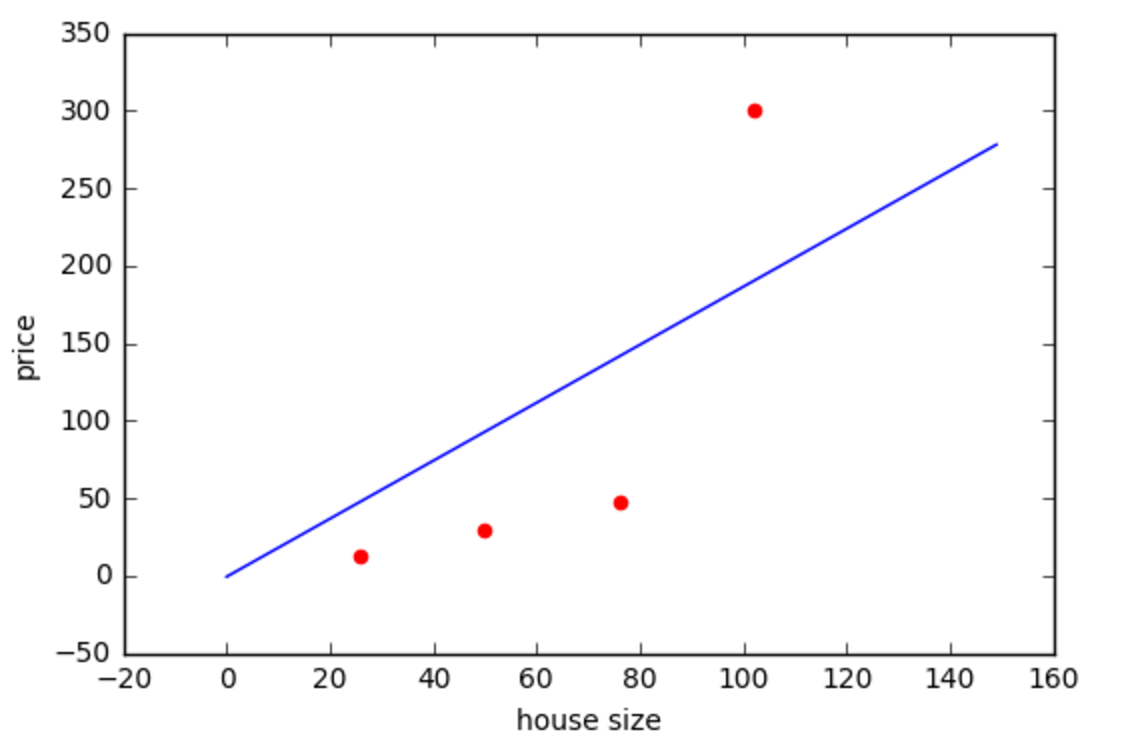
\includegraphics[width=\linewidth]{images/line_regression_outlier.png}
\end{figure}
\end{frame}

\begin{frame}{Outliers and overfitting}
When this happens, we usually notice that one of the weight is big (in this case, $\theta_1$).
\pause
\vfill
How to avoid that? \pause By penalizing big weights in the model.
\pause
\vfill 
Formally, this consists in rewriting the cost function $J(\theta)$. Initially, we had 
\begin{equation*}
J(\theta) = \dfrac{1}{2} \sum_{i = 1}^{n} \ell \left( \yhati, \yi \right)
\end{equation*}
\pause
\vfill 
We can add another term $R(\theta)$ called \textbf{regularization}
\begin{equation*}
J(\theta) = \dfrac{1}{2} \sum_{i = 1}^{n} \ell \left( \yhati, \yi \right) + \lambda R(\theta)
\end{equation*}
\pause
\vfill
where $\lambda$ is a \textbf{hyper-parameter} that quantifies how much we want to penalize big values of $\theta$.
\end{frame}


\begin{frame}{Outliers and overfitting}
In the end, $J(\theta)$ is as follows:
\begin{equation*}
J(\theta) = L(\theta) + \lambda R(\theta)
\end{equation*}
where 
\begin{itemize}
	\item $L$ is the loss term
	\item $R$ is the regularization term
\end{itemize}
\pause
\vfill
A commonly used regularization term $R$ is often the squared $\ell_2$ norm given by
\begin{equation*}
R(\theta) = \norm{\theta}_2^2 = \sum_{j = 1}^d \theta_j^2
\end{equation*}
\end{frame}

\begin{frame}{$\ell_2$-regularized OLS}
OLS with this regularization term becomes:
\begin{equation*}
J(\theta) = L(\theta) + \lambda R(\theta)
\end{equation*}
\vfill
\pause
Now, we have to work
\end{frame}

\begin{frame}
	\center
	\huge{Model evaluation\\ Parameter selection}
\end{frame}

\begin{frame}{Train-test split}
As we saw with OLS, ML algorithms usually rely on \textbf{many parameters}. How to \textbf{tune} them properly given a data set?
\vfill
\pause
The most commonly used principle is the \textbf{train-test split}:
\begin{itemize}
	\item \textbf{Split the data} into a training set and a test set
	\item \textbf{Train} on the training set
	\item \textbf{Test} on the test set
\end{itemize}
\vfill
\pause
This is often referred to as \textbf{cross-validation}.
\end{frame}

\begin{frame}{Cross-validation}
Standard technique: Hold-out cross-validation:
\begin{itemize}
	\item Train on a part of the data (e.g. 70\%)
	\item Test on the remaining data (e.g. 30\%)
\end{itemize}
\pause
\vfill
Another standard technique: \textbf{$k$-fold cross-validation}
\begin{itemize}
	\item Split the data into $k$ (equally-sized) folds
	\item Remove 1 fold (= test fold)
	\item Train on the other folds
	\item Test on the removed fold
	\item Do it for all the folds
\end{itemize}
\end{frame}

\begin{frame}{Small data set}
Suppose you have \textbf{a small data set}. How to evaluate a classifier in this case?
\vfill
\pause
$k$-fold cross-validation? Even with $k = 2$, it would make the training set even smaller and make it hard to fit a proper model.
\vfill
\pause
Other option: \textbf{Leave-one-out} (LOO) cross-validation:
\pause
\begin{itemize}
	\item \textbf{Remove 1 sample} from the data set
	\item Train on \textbf{all the other samples}
	\item Test on the sample you've removed
	\item \textbf{Evaluate} the prediction
	\item Do it \textbf{for each sample of the data set}
	\item \textbf{Aggregate} the evaluations
\end{itemize}
\pause
\vfill
\textbf{Remark}: This could lead to many iterations even if the data set is small.
\pause
\vfill
\textbf{Alternative}: Leave-$p$-out (LPO). LOO is LPO with $p = 1$.
\end{frame}

\begin{frame}{Parameter selection}
One of the goals of model evaluation is to select a \textbf{good model}.
\vfill
\pause
Hence we want to choose one (or several) parameters. How do we do?
\vfill
\pause
Most classic way: a \textbf{grid-search}
\begin{itemize}
	\item For each parameter, define a set of possible values
	\item For each parameter combination, train/test the model
	\item Pick the parameter combination which gives best results
\end{itemize}
\vfill
\pause
\textbf{Important note}: Hyper-parameter ranges vary a lot from an application to another. It is \textbf{data-dependent}.
\end{frame}

\begin{frame}{Grid search vs random search}
Random search is a more and more popular alternative to grid search, especially in this case:
\vfill
\pause
\begin{figure}
\centering
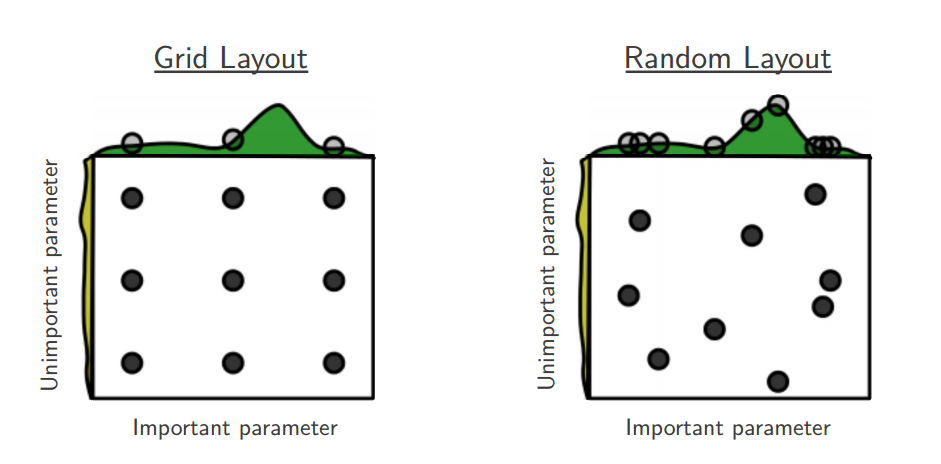
\includegraphics[width=\textwidth]{images/random_search.png}
\end{figure}
\pause
\vfill
In any case, you need to guess upper/lower bounds on the parameters.
\pause
\vfill
\textbf{Practical note}: Each parameter combination can be trained/tested separately =$>$ possibility to distribute the tasks
\end{frame}

\begin{frame}{Conclusion}
In this lecture, we've seen:
\begin{itemize}
	\item How to avoid overfitting by regularizing the model
	\item How to evaluate models
	\item How to tune parameters automatically
\end{itemize}
\vfill
\pause
During the next lecture, we will work on implementing regularization to the OLS algorithm and cross-validating it and switch to classification if the time allows it.
\end{frame}

\begin{frame}
	\center
	\huge{Thank you! Questions?}
\end{frame}

\end{document}